
1. Introduction   

% Waking up the sleeping dragon. The little Hobbit Describing the dragon.
% Drache, der alle dreissig Jahre auftaucht, seinen heissen Atem verbreitet und wieder einschläft.   

Dealing with a high risk technology such as a nuclear power plant is like dealing with a sleeping dragon in an golden cave. \footnote{Reading the little Hobbit from Tolkin, describing Smaug the dragon sleeping in the mountain covered with gold.}  Don't wake him up, do not disturb his sleep - keep him calm, cool him down, covered with gold. Once they are awake you can't control him so easy. They start to spread their poisoned air.  

 
The use of modern technologies shows that modern societies are more vulnerable because of growing dependencies and interdependencies (Jaeger et al 2001 p. 9). Technologies like nuclear power are essential to provide the power we need to build further wealth and keep economy growing. The price of technology is a society that has to deal with technologies unintended risk's or as Ulrich Beck calls it a life in the risk society (1992). And in fact, even if life improved in the past in many ways (Freudenburg 2001 \citep{Freudenburg:2001cs}), the consequences of our technological improvements for future generation remain unsolved. 

The accident in Fukushima 2011 made clear that the accident in Chernobyl 1986 was not an isolated event unlikely to recur but showed that the occurrence of an nuclear accident is always possible. Even the Fukushima disaster was a man-made disaster for the authorities failed to prevent safety requirements, because with a good safety culture the earthquake and the tsunami where foreseeable UMSTÄNDE und man hätte Schutzmassnahmen aufnehmen können  (Pidgeon 2012 \citep{Pidgeon:2012ud})  (Poortinga et al, 2013 \citep{Poortinga:2013gt}, Funabashi and Kitazawa, 2012 \citep{Funabashi:2012fs}). 

% Besonderheit nuclear Accidents
Nuclear accidents are perceived as very dangerous because they combine all undesirable characteristics of a hazard. They are uncontrollable, caused by others, can happen anytime with no time to prepare, there is not so much knowledge how to protect the BEVÖLKERUNG after an accident. (Slovic et al (1981) ( \citep{Slovic:1981fe}; Renn and Zwick (1997) (\citep{Renn:1997tx, Slovic:1981fe}).   


% Research Question
Our research question is: What are the factors influencing individuals risk perception. Do we observe a risk-gap in the society. How did the accident change the impact of social factors? Do we observe a common sense of risk among people in different countries? We think that social status is an important factor in shaping individual's risk perception (Pampel 2011 \citep{Pampel:2011cx}). Given the specific characteristic of the risk [BEGRIFF: Hochrisikotechnologie], trust authority plays an important role in forming someones risk perception.


% Studies on impact of nuclear accidents (Fukushima and Chernobyl) 

2. The impact of nuclear accidents on attitudes towards nuclear power.

Since the nuclear accident a few studies analyze the impact of Fukushima's nuclear accident on attitudes towards nuclear power like risk perception or acceptance of this technology.  
Visschers and Siegrist (2012) and Visschers and Wallquist (2013) \citep{Visschers:2012bf,Visschers:2013ee}  report a negative impact on acceptance of nuclear power after the Fukushima accident. A survey conducted in Britain and Japan (Poortinga et al, 2013) \citep{Poortinga:2013gt} does not show any change in people's acceptance of nuclear power in Britain but lower acceptance in Japan. Prati and Zanti (2013) \citep{Prati:2013jc} report lower trust in technology and a change in claim that an accident has the potential to change value orientation especially for altruistic values.
Siegrist et al (2014) \citep{Siegrist:2014ji} show that people with an increase risk perception after the accident have lower acceptance of nuclear power in Switzerland. An international study an
The Fukushima effect is similar to the decreasing acceptance of nuclear power after the Chernobyl fallout (Eiser et al., 1990) \citep{RichardEiser:1990iw} but studies analyzing the long-term effect of the accident indicates that after the immediate decrease of acceptance the acceptance of nuclear power did increased again (Renn 1990) \citep{Renn:1990kf}.  


3. Conceptualizing of risk and risk perception.

%%%%%%%%%%%%%%%%%%%%%%%             
                                                       
 


Risk is a term to deal with uncertain outcomes in the future.  Humans are embedded in an uncertain environment because of human behavior or natural circumstances.   

``Risk is defined as the possibility that an undesirable state of reality (adverse effects) may occur as a result of natural events or human activities'' (Kates et al, 1985 p.21, Zitiert in Renns Buch Risk Governance 2008 p.98) (Rosa, 1998)

Risk, in our view is not neutral, implies that the outcome has a negative impact for something of human value and is not related to an opportunity of an desired outcome (Jaeger et al 2001).

Risk judgement always implies a anticipation of future outcomes and is the basis for decisions even if the outcomes are uncertain.  


``Risk perception, in general, denotes the processing of physical signals and/or information about potentially harmful events or activities, and the formation of a judgement about seriousness, likelihood and acceptability of the respective event or activity.''   \citep[98]{Renn:2008wq}     

Individual's risk-perception, is a subjective evaluation of probability and outcomes since the judgement of the (negative) consequences and the probabilistic judgement depend on various factors based on experience, knowledge, emotions and values.        
 
Risk perception from a economic point of view analyzes the functional relationship between probability of the event or situation and its individual utility. 
Rational actors like to chose between possible options and to evaluate alternatives and choose the alternative that maximize their subjectively expected utility (Jaeger et al 2001 \citep{Jaeger:2001wv}; Renn, 2008 (Chapter 1) \citep{Renn:2008wq}).
Hence, a risk judgement is a judgement about the desirability of outcomes (Jaeger, 2001 p 18).  
Because risk in our definition is related as negative outcome, risks are perceived as expected utility losses that result from an event or human activity.
  
Individual's expected utility ($E(U)$) is a functional form of an outcome ($X$) expressed as utility ($U(X)$) weighted with an uncertainty component expressed as a probability ($p$) that the outcome will occur.  

\begin{equation}
   E(U) =  p \cdot U(X)  \nonumber
\end{equation}
The probabilities are in the range between 0 and 1 ($0 \leq p \leq 1$). It also implies that  an event $X$ has the probability $p$ that it will occur and the probability $1-p$ that its compliment will occur.  

The rational actor paradigm  implies that people maximize their utility ($E(U)$). It does not specify how people evaluate their probabilities or how they measure utilities. 

We assume that individuals base their probability judgement on the available information. The information and the probabilistic process differs between individuals. The probability (p) of an uncertain event (X) is conditioned on the information (e): p(X|e) (Morgan and Henrion , 1990 p49) ( Fischoff 1981, \citep{Fischhoff:1981tx} [habe ich von Renn 2008 p19]).  Hence subjective probabilities in this sense are the degree of belief in the occurrence of an event, that a person has at a certain time with a given set of information  (de Finetti, 1974 \citep{deFinetti:1974ua}).  
Assuming that an nuclear disaster has the same negative utility for everybody (U(nuclear accident)) there are different probabilities because people may have different information about the occurrence of an uncertain event. The same person may also change his' or her's probabilities over time if new informations are available.

4. Change in individual's risk perception

 According to the idea of subjective probabilities we assume that the Fukushima accident changed the assumption that a new accident will occur in the future. After the Fukushima accident the probability assumption (p(X|e)), that an nuclear accident will happen in the future is based on the past knowledge of two major accidents since 1986 (p(X|Fukushima and Chernobyl). This a-posteriori probability should be higher than the a-priori knowledge of only one accident p(X|Chernobyl).    

Even if the probabilities of an accident in the future remains quite low, the high catastrophic potential  of a possible accident shapes individual's risk-perception (Slovic, 2000, p148f) [CHECK REFERENCE weil ich 2001 aufgeschrieben hatte]   \citep[148]{Slovic:2000tx}. That means even a small change in the [EINTRITTSWAHRSCHEINLICHKEIT] probabilities of an accident, increases individual's risk perception because of the catastrophic potential of a future disaster. 

People also use heuristics to simplify the evaluation of a negative outcome. The evaluation not always implies all available information and can be influenced by emotions and therefore can differ between individuals much even if they have the same experience. According to the availability heuristic  (Tversky and Kahnemann, 1974; Kahnemann and Tversky, 1979; \citep{Tversky:1974wi,Tversky:1973ui, kahnemann_prospect_1979}) people overestimate the probability of a similar event if a event just happened and is easy to remember. The affect heuristic  (Slovic et al, 2004; Slovic, 2000 \citep{Slovic:2004hj}\citep{Slovic:2000tx}) (Finucane et al, 2000 \citep{Finucane:2000wu}) emphasis the context of an risk. If people have a negative feeling of a situation they overestimate its probability. Emotions become more important by judging a risk, if people don't have enough opportunities to analyze the situation. Both heuristics bear evidence that after an accident people should have a higher risk perception because the information is in the press and people are more aware of the negative consequences and problems we have to deal with the accident even if they have not been affected directly by the accident because they live geographically apart.  

Our theoretical explanations to support our hypothesis of a overall increase in risk perception after the Fukushima accident do not exclude an non-change or decrease of individual's risk evaluation. Even with an increase in probability, an decrease is still possible if the consequences of the accident are not as severe than a-priori expected. The way governments reacted to the crisis and passed as a result new laws like the ATOMAUSSTIEG in Germany or Switzerland to protect citizens and to reduce risk in the future can rebuild trust and are influencing individual's risk perception.        

For the functional form of risk perception we furthermore assume that there is no linear form in risk perception but a concave form (BEGRÜNDUNG XXXX LITERATUR?). That means that the change in average risk perception because of additional information after the accident depends on the overall level before the accident. In the extreme case of someone who beliefs that a nuclear accident will happen in the future the information that this event happened is not changing the degree of belief (probability) very much again but only confirms the a-priori risk-awareness. Someone who was not sure about a the chance of a new accident, now has the prove that nuclear accident are very likely to happen in the future and are higher than a-priori expected and will adjust his' or her's probability assumption more drastically.  Because we have no longitudinal data of individuals we only can test our hypothesis for subgroups not individuals. Our hypothesis therefore is: for subgroups of the population like that subgroups with on average a higher risk perception before the disaster should have a lower increase  compared to subgroups that had on average a lower risk perception before the accident. 

It is important to understand the subjective risk-evaluating process.  All processes, bayesian updating (more information), availability heuristic (event is present),  affect heuristic (external shock) indicate an increase in people's risk perception after the Fukushima accident. 
In this paper we want to examine if the change in risk perception happened equally in the society. The main question therefore is: How did the accident change individual's risk perception? Did the accident divided societies so they became more extreme or did the incident lead to a more homogenized risk perception within societies?


    
5. Explaining differences in individual's risk perception. 

The risk evaluating process differs between individuals and subgroups in the society so that explain differences in risk perception before the accident. Research shows that sociodemographic factors influences individuals's risk judgement and lead to a per se heterogeneous risk-perception within a society. It is also the case that there are benefits from the technology that influences individual's risk-perception, like a `clean' image of nuclear power because of low CO2 emissions or a independent source of energy for the country. Individuals accept risks if the corresponding benefit adds more utility than the risk detracts from the utility (Renn, 2008 p.18f [CHECK REF AGAIN]).
 
Gender is strongly related to risk judgement. There is strong empirical evidence that women express higher levels of concern toward technology and therefore have a higher risk perception than man (LITERATUR EINFÜGEN, WELCHES KAPITEL?? - SLOVIC 2000, 396 gibt einen Überblick) \citep{Slovic:2000tx}. One explanation: Women tend to express greater concern than do man about health and safety (Davidson and Freudenberg, 1996 \citep{Davidson:1996uk}).  Males also associate nuclear power with neutral or positive attributes like energy and necessity or waste deposal, where as women rather associate negative emotions like severe accidents and environmental problems with nuclear power (Keller et al, 2011 \citep{Keller:2011gb}; Siegrist, 2014 \citep{Siegrist:2014ji};).  

Pampel (2011) \citep{Pampel:2011cx} report a higher support for nuclear energy for older people across European countries. For risk-perception we therefore assume a lower risk perception for older people because of a cohort effect. The older generation did benefit the most by nuclear technology and their values where shaped before the accidents of Chernobyl 1996 and Fukushima 2011 happened. Siegrist et al (2014) \citep{Siegrist:2014ji} report that after the accident older people had a higher chance to change from promoting nuclear technology to opposing nuclear power than younger people. [GIBT ES ANDERE QUELLEN?]       
 
Socio-economic status seems to influence individuals' risk perception negatively. The inverse relationship indicates that higher educated people as well as higher income class people tend to have a lower risk perception (Pampel, 2011; Greenberg 2009; Greenberg/Truelove 2011; Whitfield et al. 2009 \citep{Pampel:2011cx,Greenberg:2009fx,Greenberg:2011ja,Whitfield:2009ku}).  One explanation is that better educated people know more about technology (Costa-Font, 2008 \citep{CostaFont:2008hf}) tend to belief in technological development more easily and disagree that technological development is a danger for nature.  One explanation by Flynn et al. (1994) \citep{Flynn:1994dn} follows a sociopolitical argument that claims that better educated people (especially white man) to perceive less risk because they created and managed, control and benefit the most from technologies. 

% adaptation-of-risk-hypotheses 
According to the theoretical argument, that risk-perception is not a linear trend and given the assumption of a Bayesian probabilistic view, the change in risk-perception should be higher for those with on average lower risk perception. We call it the adaptation-of-risk-hypotheses due to extreme events. That means, male and people with higher social economic status should have a higher change in their risk perception as well as older people. 
 
  
Keeping in mind the nature of nuclear risks it is important to discuss the role of social trust (Keller et al, 2011; Whitfield et al, 2009; Poortinga and Pidgeon, 2003; Greenberg 2009; \citep{Whitfield:2009ku,Poortinga:2003cb,Keller:2011gb, Greenberg:2009fx} ) because scientific impact can not prevent people to have fears of low probability events like a nuclear disaster. Trust in political institutions is crucial to believe that governmental institution are able to manage technological risks today and to provide protection for those at risk in the future (Kasperson, 2008 p345 \citep{Kasperson:2008tw}).  
Trust is created rather slowly and once lost extremely hard to rebuild - a negative event can destroy trust in an instant. Negative events weight much more than positive events in building or destroying trust in technology  -- that is what is called the the ``asymmetry principle''. (Slovic, 1993 \citep{Slovic:1993gm}). [SAME article as book chapter Slovic 2000, p 320)].  
After the Fukushima accident people who still report to trust the government, should express a lower risk perception compared to people that did not trust the government. After the accident the reporting in the media about the negative consequences are very obvious, also the lack of scientific knowledge and technical details of how to solve the problem. If after the Fukushima event someone still trust the government, that also means, that they belief the government proved their ability to manage the situation well and will protect society. So the effect should get stronger after the disaster.

    
% if we want to add political orientation: People who express less risk perception also are more conservative.[LITERATURANGABEN DAZU im Sammelbandbeitrag von mir]

6. Data and Methods 

% ISSP Dataset
% Operationalisierung der Variablen 
% Daten in Stichprobe vor und nach dem Unfall. Tabelle mit Fallzahl spezifizieren. 

% Fixed Effects Model
%   Kontrollvariablen: Zeit und Land

% Für die Prüfung der Hypothesen verwenden wir Daten des International Social Survey Programmes (ISSP) 2010 Environmental Module (QUELLE ISSP EINFÜGEN). Die Daten wurden in XX Ländern im Zeitraum von XX bis XX erhoben (Für eine genaue Darstellung der Erhabungszeiträume siehe Abbildung XX). In allen Befragungsländern wird ein einheitlicher Fragebogen mit 60 Umweltspezifischen Fragen gestellt. Der Fragebogen wird meist im face-to-face CAPI interviews geführt, aber auch teilweise mit CATI-Telefoninterviews  per Fragebogen erhoben [GUT WÄRE HIER EINE TABELLE MIT GENAUEM BEFRAGUNGSZEITRAUM; INTERVIEWMETHODE; BEFRAGTE VOR UND NACH FUKUSHIMA]. In der Stichprobe vor dem 11.3. 20111 befinden sich XX Befragte aus XX Ländern. In der Stichprobe nach dem 11.3.2011 befinden sich XX Befragte aus XX Ländern. In XX Länder fällt der Unfall innerhalb des Befragungszeitaum, so dass hier Personen vor und nach dem Unfall befragt wurden [BRACHEN WIR DIE INFO?]. In die Analysen fliessen nur diejenigen Befragten ein, die sicher entweder vor oder nach dem Unfall eingeordent werden können. Befragte aus Canada, die im MÄrz befragt wurden, werden aus den Analysen ausgeschlossen, da nur Monatsgenaue angaben über den Befragungszeitraum vorliegen [WERDEN NOCH WEITERE AUSGESCHLOSSEN].

% Das Risikobewusstsein wird durch die Frage: XX operationalisiert. Befragte können auf einer fünfstufigen Likertskala angeben ob sie XX .... XX gefährlich finden. Der Wertebereich der Variable beträgt daher 1 bis 5. 
% [Tabelle XX mit Variablen-Kennzahlen einfügen]
% Die Soziodemografischen Variablen sind folgendermassen operationalisiert. Geschlecht ist eine Dummy-Variable mit Männlich als Referenzkategorie. Das Alter ist eine metrische Variable im Altersbereich von XX bis XX. 
% Die Bildung einer Person ist in 6 Kategorien erhoben mit ``keine Bildung'' als Referenzkategorie. 
% Vertrauen ist eine Variable die auf  einer [??] Likertskala erhoben wurde. Personen können zum einen angeben, ob sie den PErsonen allgmeien Vertrauen (Allgemeins Vertrauen) und ob sie Menschen Fair finden. [GENAUE OPERATIONALISIERUNG NOCH NACHSCHAUEN] 
% [VERTRAUEN IN REGIERUNG AUCH NOCHMAL GENAU ANSEHEN].

% ANALYEMEHTEODE  


7. Results 
\begin{figure}[h!] % input Graph hier, Option t für "on top"
  \begin{center}
    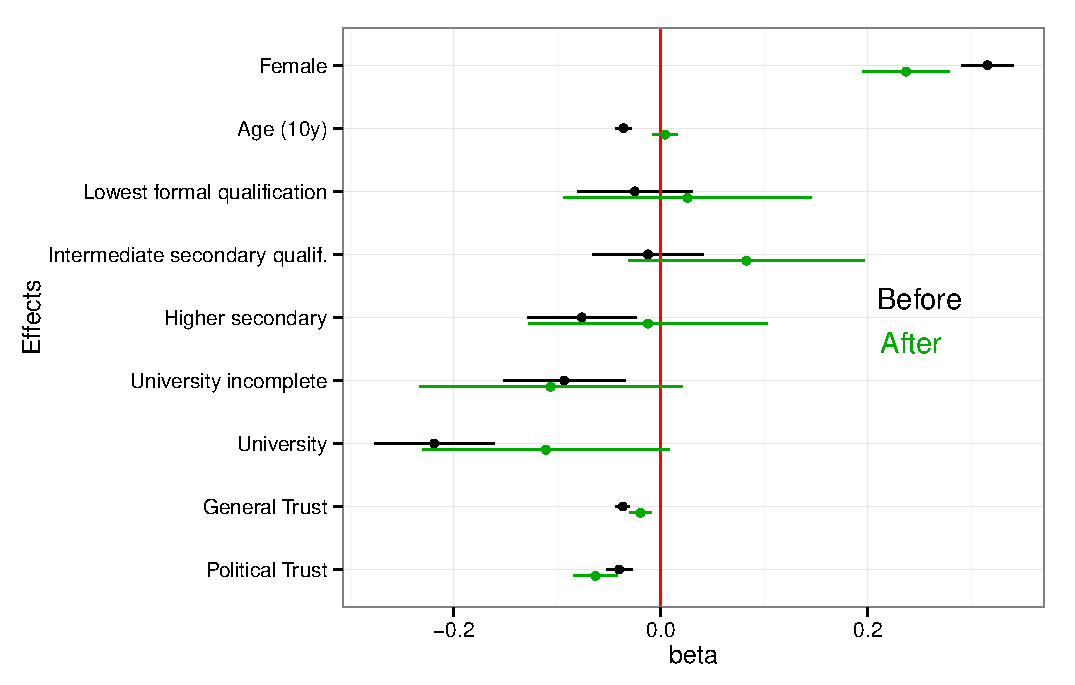
\includegraphics[width=0.67\textwidth]{images/results.pdf}
  %  \caption{}
  %\label{fig:}
 \end{center}
\end{figure} 
% Einleitungssatz: 
% Die Resultate des Fixed-Effects-Modells in Abbildung XX (Tablle XX im Anhang) bestätigen die Ausgangshypothese, dass das soziale Faktoren das Riskobewusstsein beeinflussen. Es wird ferner die Hypothese bestätigt, dass der Unfall zu einer Angleichtung des Riskobewusstseins innerhalb der Bevölkerung geführt hat und nicht zu einer Radikalisierung. 

To test the hypotheses two separate we perform two regression analysis. The first sample only includes respondents [BEFRAGTE?] that were conducted before March 11th, 2011. The second sample includes respondents that were asked after the accident.   
The fixed effects models of both samples, as displayed in Figure XX (see also for exact figures Table XX in the appendix) confirm the general hypothesis that social factors influence risk perception systematically. Furthermore, we can prove the hypothesis, that after the accident people adapt a more unified risk perception.   


% Erklärung der Grafik. 
% Die Abbildung XX zeigt, den Zusammenhang des Riskobewusstsein mit den, in Abschnitt XX [Daten und Methode] spezifizierten sozialen Einflussfaktoren für Befragte vor und nach dem 11. März 2011. Der Koeffizient zeigt die Veränderung der Riskoeinstellung im Wertebereich von 1 bis 5, wenn sich der soziale Faktor um eine Einheit erhöht, die horizontale Linie um den Effekt zeigt das 95% Konfidenzintervall. Positive Effekte bedeuten ein höheres Risikobewusstsein. Wenn der Einflussfaktor nach der Messung einen geringeren Effekt hat, dann interpretieren wir das als eine Abschwächung des Effekts, der durch den Unfall hervorgerufen wurde. 
Figure XX shows the relationship between risk perception and sociodemographic factors as explained in Chapter XX [Data and Methods] for respondents before and after the Fukushima accident. The regression coefficient, depicted as a point, describes the change in risk perception if the independent variable changes one unite. The horizontal line describes the 95 Percent confidence interval. If the confidence interval includes the horizontal zero line, there is no significantly different relationship. 
Positive effects indicate a higher risk perception, negative effects a lower risk perception. After the accident, if the positive or negative effect is closer to zero than before the accident, that indicates that risk perception in society got more homogenized after the accident.   

% Frauen haben ein höheres Riskobewusstsein und der der Effekt nach dem Unfall geringer (von XX auf XX). Die (signifikante) Abschwächung des Effekts für Frauen deutet darauf hin, dass sich durch den Unfall  das Risikobewusstseins der Männer stärker erhöht hat als für Frauen. Frauen damit auch noch nach dem Unfall ein höheres Risikobewusstsein haben, der Effekt allerdings nicht mehr so stark ist. 

In both sample, as assumed, women have a higher risk perception. The gender effect for women is not as high anymore after the accident. The significant decline indicates that after the accident men's risk perception increased more drastically than women. [T-TEST PROOF of gender level before and after 3/11] Women still have a higher risk perception but the effect is not so strong anymore - evidence that the accident led to a more unified [VEREINHEITLICHTE] risk perception.  
%[WAS WIR BRAUCHEN IST EINE T-WERT TABELLE MIT DEN DURCHSCHNITTSWERTEN NUR FÜR VORHER-NACHHER GRUPPEN.]

% Vor dem Unfall nimmt mit steigendem Alter das Risikobewusstsein ab (pro 10 Jahre um XX Punkte). Dieser Effekt lässt sich nicht für die Befragten nach dem Unfall beobachten - Alter hat nun keinen Einfluss mehr. Auch beim Alter beobachten wir  - der ``Anpassungs''-Hypothese entsprechend - eine Anpassung des Riskobewusstseins innerhalb der Altersgruppen in der Bevölkerung.

Before 3/11 risk perception decreased with older age [HÖHEREM ALTER] (per 10-years XX index-points). There is no significant age effect for the post accident sample. We therefore find evidence that beside men also older people adapt their risk perception stronger [?? etwas stärker anpassen: to adapt stronger??]   

% Der Soziale Status - gemessen in der Bildung - zeigt die erwarteten negativen Effekte für besser gebildete Personen. Im Vergleich zur Referenzkategorie der Nicht-gebildeten, haben  Personen mit einem Bildungsstatus von mindestens ``higher secondary'' ein niedrigeres Risikobewusstsein.  Der Bildungseffekt ist nach dem Unfall nicht mehr signifikant und zeigt auch, dass besser gebildete Personen nun im Mittel kein niedrigeres Risikobewusstsein mehr zeigen. 

Education, an indicator for social status, has the expected negative effect on risk perception for better educated people. Before the accident, compared with the reference category ``no formal education'', people with an at least ``higher secondary''  education have a lower nuclear risk perception. E.g. individuals with an ``university degree'' have a XX points lower risk perception. The effect decreases after the accident and is not different from the reference category anymore. This is also evidence in favor of the [adaptaion-after-accident-] hypothesis.

% VERTRAUEN _ GENAUE OPERATIONALSIERUNG NOCHMALS CHECKEN _ OB METRISCH ODER DUMMY: Die Vertrauenseffekte sind einheitlich negativ, was darauf hindeutet, dass Personen, die ein höheres allgemeines Vertrauen als auch ein höheres Vertrauen in die Regierung haben ein niedrigers Risikobewusstsein haben. Interessanterweise hat der Unfall einen gegenläufigen Effekt für das Vertrauen. Der Effekt bleibt immer noch negativ, allerdings kommt es nur beim allgemeinen Vertrauen zu einer Anpassung der Einstellung. Für die Personengruppe, die nach dem Fukushima Disaster, Vertrauen in die Regierung ausdrücken, hat sich der negative Effekt verstärkt. Der stärkere negative Zusammenhang deutet darauf hin, dass diese Personengruppe nun aufgrund ihres Vertrauens in die Regierung die Atomenergie als eine weniger gefährliche Technologie betrachten. 

% VERTRAUEN _ GENAUE OPERATIONALSIERUNG NOCHMALS CHECKEN _ OB METRISCH ODER DUMMY: 
Both effects of general trust and trust in governance are negative indicating that trust decreases risk perception towards nuclear power. Interestingly enough the effect of trust changes differently after the accident. On the one hand people who tend to trust people more still have a lower risk perception but this effect is not as clear anymore. On the other hand, people who trust government more after the accident now have an even lower risk perception than the individuals trusting the government before the accident. The increased negative relationship indicated that people who trust the government got more radical and compared to other people perceive nuclear power as less dangerous. [ES IST EINE RELATIVE VERÄNDERUNG ODER IM MITTEL KÖNNTE AUCH HIER DIE RISIKOEINSTELLUNG HÖHER GEWORDEN SEIN - ABER EBEN EXTREMER GETRENNT?? HABEN WIR SEPARATE MITTELWERTE FÜR before AND after PRO LAND?]





% Schlusssatz: ZUSAMMENFASSUNG: 
% Der Zusammenhang von Risikoeinstellung und den beoachteten Soziodemographischen Merkmalen zeigt, dass vor dem Unfall Männer und Personen höheren Alters, besser gebildete und Menschen mit höherem Vertrauen, jeweil ein geringeres Riskobewusstsein gezeigt haben. Diese Effekte verringern sich gemäss der Anpassungshypothese nach dem Unfall. Vertrauen in politische Institutionen wie die Regierung hat lediglich einen starken risikoverringernden Effekt und bestätigt die Trust-in-Institution-Hypohtese. 

To summarize the findings. The relationship of risk perception and the social factors reveals clearly that after the accident men, older people,  people with better education and those who trust more in people changed their risk perception [STÄRKER] more drastically. Therefore the perceived differences in risk perception decline after the accident. This results are in line with the adaptation-after-risk-hypothesis. There is one effect that shows the opposite. Individuals who trust in governance after the accident did not adapt their risk perception and now show an even stronger decline in risk perception. 







% Conclusion:  

Die Ergebnisse der Studie geben Licht in die Risikoeinschätzung der Bevölkerung.    
Wir konnten auch zeigen, dass es nicht nur ein perception gap zwischen Experten und Laien gibt (vgl. Slovic et al 1982), sondern auch ein perception gap in der breiten Bevölkerung. Unsere Ergebnisse zeigen, dass  Männern, ältere Menschen und besser gebildeten Personen ein geringeres Risikobewusstsein haben. 

Vor dem Reaktorunfall gab es schon eine heterogene Meinung über die Gefahren der Atomkraft. Damit zeigt sich, dass es Bevölkerungsschichten gibt die die Atomenergie tendenziell als gefährlicher oder weniger gefährlich eingeschätzt.   
Interessanterweise sind es die tendenziell politisch und sozial benachteiligten Bevölkerungsschichten, Frauen, junge Menschen und Menschen mit geringerer Bildung, die ein höheres Riskobewusstsein zeigen. 

Die Frage die sich daran anschliesst ist, ob der Atomunfall das perception gap erweitert hat oder nicht. Kam es zu einer Radikalisierung oder Solidarisierung der Bevölkerungsschichten eines Landes bei der Beurteilung der Gefährlichkeit der Atomenergie? Wir stellen die `adaptation-after-accident-Hypothese' auf [oder sollen wir es die Solidarisierungshypothese/Homogenisierungshypothese durch eine Katastrophe nennen?]

Die Ergebnisse zeigen, dass sich die Risikoeinstellung innerhalb der Gesellschaft angeglichen hat. Relativ betrachtet zum durchschnittsniveau innerhalb eines Landes. Es kam zu einer Vereinheitlicheung udn Anpassung, so dass es eine höhere Solidarität innerhalb der Gesellschaft gibt. 


Wie sehr soll die Meinung in der allgemeinen Bevölkerung nach der Reaktorkatastrophe von Fukushima beachtet werden? Kurzfristige Effekt konnten wir direkt nach der Reaktorkatastrophe beispielsweise in Deutschland erleben, wo es zu einem Vertrauensverlust in die Regierung kam und dieser erst durch den politischen Beschluss eines Atomausstiegs (Energiewende) wieder gewonnen wurde. Das Katastrophenpotential der Nukleartechnologie und die Risikoeinschätzung, die durch die availablility und affect heuristics [NOCH BESSER AUSDRÜCKEN, WIE DER MECHANISMUS IST. bilder, negative emotionen etc...] sicherlich beeinflusst wurden haben die Meinung kurzfristig stark beeinflusst. 

Allerdings bekräftigen die Fakten von zwei Unfällen in den letzten 30 Jahren, dass die Besorgnis in der Bevölkerung, wenn sie auch aus theoretischer Sicht noch so irrational erscheinen mag, berechtig ist und dass ihr Beachtung geschenkt werden sollte (Slovic et al 1982, p. 487). Die Bevölkerung, nicht die Experten haben ein realistischers Bild über die wahre Chance eines Unglücks. 
Die DIskussion über die Wahrscheinlichkeit eines Unfalls erscheint bizarr, angesichts der Tatsache, dass man von sehr geringen Wahrscheinlichkeiten spricht. Hier hilft auch die Terminologie der Wissenschaft, wahre Gefahren zu vertuschen, weil das Risikoassessment mit grossen Annahmen arbeitet. Menschliches Versagen, schlampige Kontrollen und eine fehlende Risikokultur kann man nur mit grosser Unsicherheitstoleranz modellieren und lässt Spielraum für eine Ideale Welt einer unfallfreien Atomenergiegewinnung. Unser Ansatz, der von einem Bayesian Updating spricht, scheint uns zwar eine simple Vereinfachung der Riskoeintscheidung zu sein, aber eine, die nur die Tatsachen berücksichtigt und zeigt, dass die Bevölkerung das Risiko (auch vor der Katastrophe) nicht irrational eingeschätzt hat. Mit der objektiven Wahrscheinlichkeitseinschätzung besitzen wir ein Tool, um die Gefahren zu verschleiern (Eintrittswahrscheinlichkeit 1/1000 - wer soll hier die unabhängigen Ereignisse verstehen, es kann morgen oder in 1000 Jahren kommen, beides ist gleich wahrscheinlich.) Die subjektiven Wahrscheinlichkeiten vereinfachen extrem zwei Unfälle in 30 Jahren (2/30). Also gehe ich davon aus, dass in den nächsten 30 Jahren wieder so ein Ding in die Luft geht. Laien, die so denken überschätzen die Gefahr in keinster Weise. 

Reaktorunfälle sind auch eine Gefahr für Regierungen, weil zur Unterstützung in Hochrisikotechnologien (unkontrollierbarkeit etc. WEITERE ANGABEN) das Vertrauen in die Regierung ein entscheidender Faktor ist. Vertrauen wird langsam aufgebaut und kann sehr schnell zerstört werden. Auch politische Entscheidungen wie der Atomausstieg in einigen Ländern ist daher keine irrationale oder übertriebene Antwort auf die Reaktorkatastrophe. Warum allerdings der Atomausstieg nur in einigen Ländern geschah, warum manche Ländern ruhig blieben, dass ist Gegenstand weiterer Forschung.  

Unsere Argumente führen zu dem Schluss, dass Laien auch bei der Anerkennung von Risikotechnologien in den Entscheidungsprozess mit einbezogen werden sollen. Laypeople should somehow be included in the decision-making process. Even if their perception might be quite different from experts. 

Experten können dazu dienen die Risiken zu minimieren, es bleibt aber immer ein Restrisiko. Die Akzeptanz des Restrisikos ist eine politische Entscheidung. Es bleibt zu diskutieren, ob die Bevölkerung durch bspw. Volksentscheide zum Bau neuer Atomkraftwerke über das Restrisiko mitentscheiden darf. 
    
Die empirische Evidenz zeigt, der nächste Unfall kommt mit grosser Sicherheit, welches Atomkraftwerk es trifft und was die Gründe sein werden bleibt gering. Fakt ist wir können die Kraftwerke nicht sicherer machen, denn gegen die Sicherheit spielt der Faktor Zeit und die lange Laufzeit der Atomkraftwerke und Systemversagen durch Akteure oder unvorhergesehene Naturereignisse. 
    
Die intensive Förderung CO2-arme Energiegewinnung, die unabhängig von Nukleartechnologie ist unbedingt notwendig, um auf die politischen Folgen, wie die Forderung nach einem raschen Atomausstieg, des nächsten Unfalls vorbereitet zu sein. 
   


%Limitation of the study: 

Die Studie hat auch Grenzen ihrer Aussagekraft (Limitations). Der Fukushima-Effekt wird nicht durch eine Längsschnittstudie gemessen, so dass keine Aussagen für Individuen, sondern nur Vorher- Nachhervergleiche für aggregierte Subgruppen getroffen werden können. Im Vergleich zu Siegrist (2014) wird auch nicht nach der Akzeptanz von Nukleartechnologie gefragt, einem Konzept, dass die Risken als auch die Benefits berücksichtigt. Die Schweizer Studie zeigt, dass eher die Benefits als die Risiken die Akzeptanz von Kernenergie beeinflusst. Inhaltlich haben wir uns auch auf den Zusammenhang von soziodemographischen Variablen wie Geschlecht, Alter und Bildung beschränkt sowie den Einfluss von Vertrauen erörtert. We did not address moral norms like (de Groot and Steg, 2010 \citep{deGroot:2010ez}) or worldviews (Flynn et al. 1994 ). 
Wir haben auch nur Daten für eine mittelfristige Periode und können keine Aussagen über die Langzeitveränderung der Risikoeinstellung zur Kernenergie treffen. Renn (1990) shows that Chernobyl only had a short-term impact, gleiches könnte auch für Fukushima gelten.                                         
      

% Hypothesen Zusammenfassung.    




% Research question. 


% Conclusion
% In diesem Paper verstehen wir  Risk Perception nicht im traditionellen Sinne (als Funktion von objektiven Wsk und den Folgen), sondern Betrachten public concern of a risk more widly. Die Reaktionen in der Bevölkerung zeichnen ein Bild der Risikowahrnehmung, das die Senibilisierung zu Sozialen, Technischen udn Psychologischen Faktoren darstellt. (Slovic, 2000, 392) 

%  (!) Public concern is not ignorant or irrational. Public's reactions to risk can be attributed to a sensitivity to  technical, social, and psychological qualities of hazards that are not well-modeled in technical risk-assessment (e.g. qualities such as uncertainty in risk-assessment, perceived inequity (=Ungerechtigkeit) in the distribution of risks and benefits, and aversion to being exposed to risks that are involuntary not under one's control or dreaded (=gefürchtet)). (Slovic, 2000, p392)

% "We do not expect that the accident will have long-lasting effects on the attitudes formed by teenagers or young adults. The discussion about the benefits of renewables may have a negative impact on the benefit perception of nuclear power. Therefore, we cannot rule out that future generations who will start to participate in the political process in the next few years may have more negative attitudes toward nuclear power com- pared with the sample examined in the present study." (Siegrist 2014 p.6)  



%%%%%%%%%%%%% TEXTBAUSTEINE %%%%%%%%%%%%%%%%%%%%%%%
% The aim of the present study was to examine      
% to shape people's opinion                        
% Our results suggest that
% Some limitations of the present study need to be addressed.
% The present study focused on (the impact of perceived risk and perceived benefit on the acceptance of nuclear power.) 
% The study may thus provide more insights into the complex affect-laden imagery of nuclear power plants
% This can best be explained by... 


%%%%%%%%%%%%%% To Do %%%%%%%%%%%%%%%%%%%%%%%%%%%%%%%

% Quellen die efidenz für einen negativen ALTERS-Effekt melden. 





